\documentclass{beamer}

\usepackage[latin1]{inputenc}
\usepackage{tikz}
\usetikzlibrary{arrows,shadows}

\usetheme{CambridgeUS}
\logo{
\includegraphics[scale=0.1]{redhat-logo.jpg}}
\title[OpenStack Liberty Keystone Midcycle ]{ Risk Assessment and Mitigation for Access Control mechanisms in OpenStack.
}
\author{Adam Young}
\institute{Red Hat Identity Management Team}
\date{Jul 15, 2015}
\begin{document}


\setbeamertemplate{navigation symbols}{}


\begin{frame}
  \titlepage
\end{frame}

\begin{frame}{Introduction}
  \begin{center}
    \begin{exampleblock}{}
      Risk Assessment and Mitigation for Access Control mechanisms in OpenStack.
    \end{exampleblock}
  \end{center}
\end{frame}

\begin{frame}
  \frametitle{Agenda}
  \tableofcontents
\end{frame}


\section{Threat Assessment}


\begin{frame}{Hypervisor Compromise: Tokens }
  \begin{itemize}
  \item validates the token
  \item Nova Compute Runs on the Hypervisor
  \item Tokens included included in requests
  \item Rogue VM Harvest Tokens
  \end{itemize}
\end{frame}


\begin{frame}{Hypervisor Compromise: Trusts}
  \begin{itemize}
  \item Allow for a long term delegation
  \item A rogue trust would by-pass the token expiry
  \item Without Trusts, passwords will be copied around, which is even worse.
  \item Easy to identify but you have to look
  \end{itemize}
\end{frame}


\begin{frame}{Authenticate via Token when fetching a token}
  \begin{itemize}
  \item Risk
      \begin{itemize}
        \item Any scope can be converted to another scope
        \item Expiration is not extended
      \end{itemize}
    \item Why:
      \begin{itemize}
      \item Web UI does not cache password
      \end{itemize}
    \item Mitigate
      \begin{itemize}
      \item Only allow unscoped to scoped transitions
      \item Requires a call to explicitly request a scoped token
      \end{itemize}
  \end{itemize}
\end{frame}

\section {Use of Tokens }

\begin{frame}{Why Are Tokens on Hypervisor}
  \begin{itemize}
  \item Boot and Teardown
    \begin{itemize}
    \item Barbican, Glance, Cinder, Neutron
    \end {itemize}
  \item Attach (Cinder)
  \item Periodic Refresh (Neutron)
  \item Snapshot (Glance)
  \end {itemize}
\end {frame}


\begin{frame}{Why Are Tokens on Hypervisor}
  \begin{block}{}
    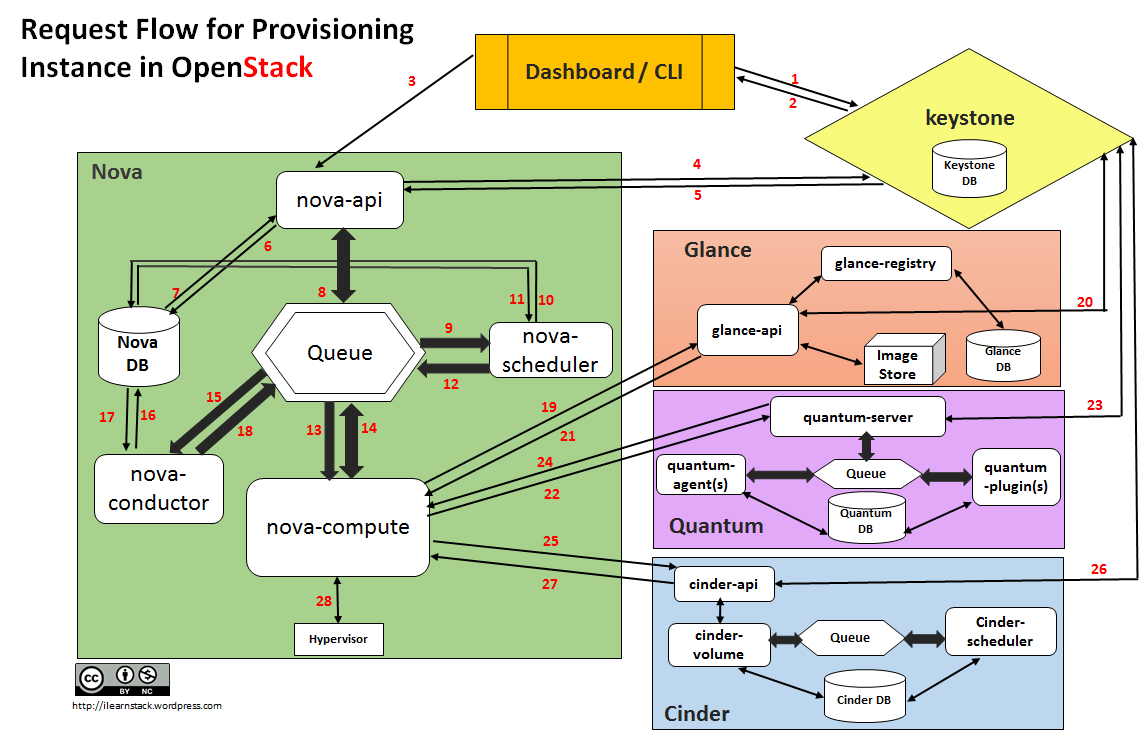
\includegraphics[scale=0.3]{request-flow1.png}
  \end{block}
  http://ilearnstack.com/2013/04/26/
\end {frame}

\begin{frame}{Trove Uses Tokens}
  \begin{block}{}
    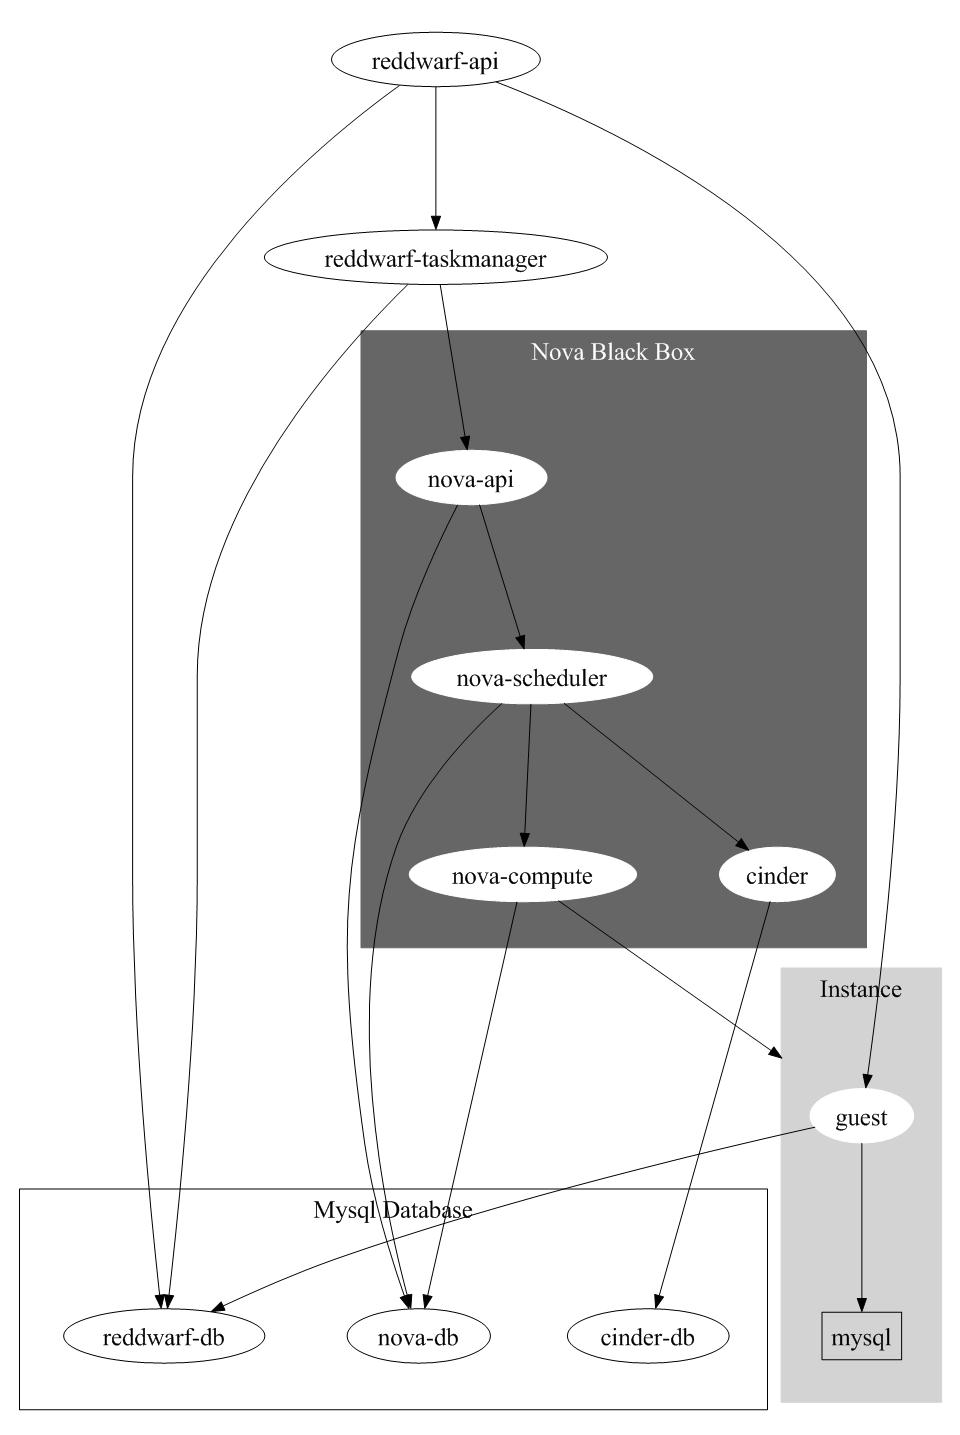
\includegraphics[scale=0.2]{Reddwarf-overview.jpeg}
  \end{block}
  https://wiki.openstack.org/wiki/Trove/trove-diagrams
\end {frame}

\begin{frame}{Sahara Uses}
  \begin{block}{}
    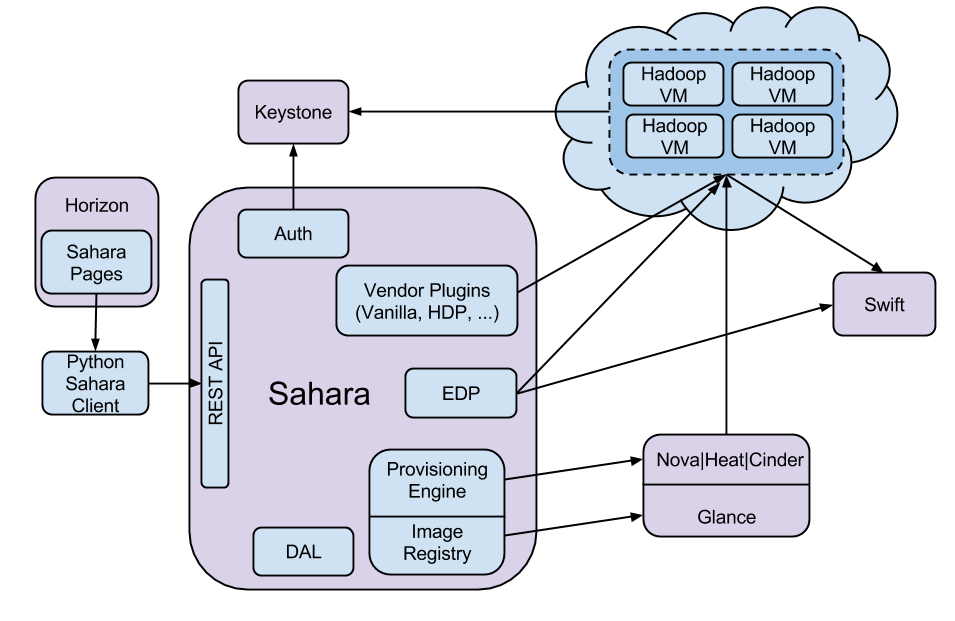
\includegraphics[scale=0.3]{sahara-architecture.png}
  \end{block}
  http://docs.openstack.org/developer/sahara/architecture.html
\end {frame}

\begin{frame}{Solum and Heat Use Tokens}
  \begin{block}{}
    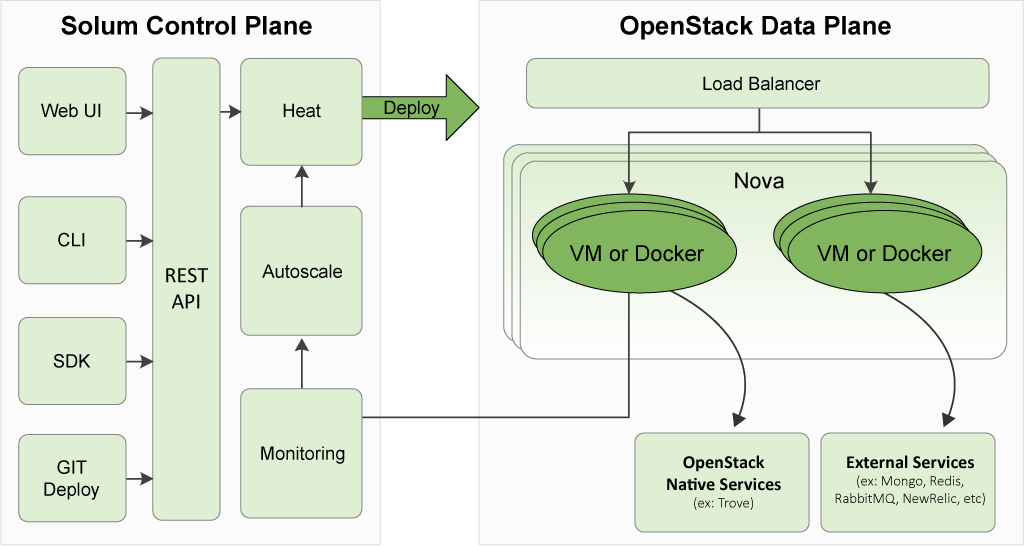
\includegraphics[scale=0.3]{solum-arch.png}
  \end{block}
  http://solum.io/img/chart.png
\end {frame}

\begin{frame}{Barbican Uses Tokens}
  \begin{block}{}
    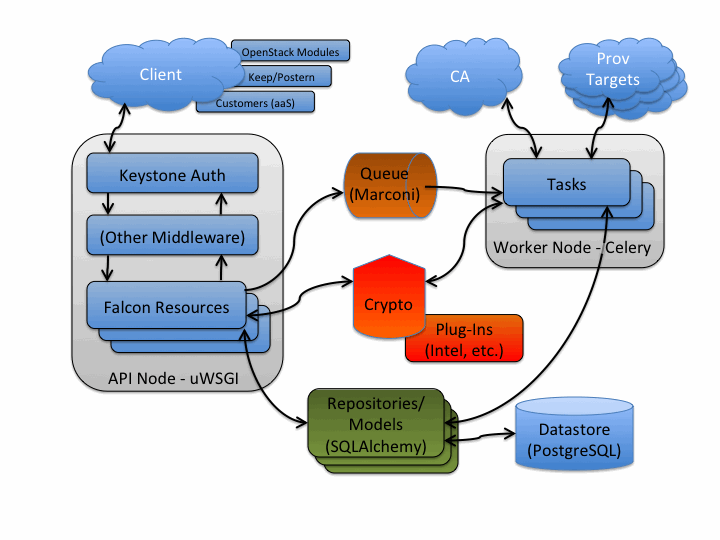
\includegraphics[scale=0.3]{barbican-arch.png}
  \end{block}
  https://github.com/cloudkeep/barbican/wiki/Architecture
\end {frame}

\begin{frame}{Big Tent Services that User Tokens}
  \begin{columns}[t,onlytextwidth]
    \begin{column}{.25\textwidth}
      \begin{itemize}
      \item Barbican
      \item Ceilometer
      \item Cinder
      \item Congress
      \item Cue
      \item Designate
      \end{itemize}
    \end{column}

    \begin{column}{.25\textwidth}
      \begin{itemize}
      \item Glance
      \item Heat
      \item Horizon
      \item Ironic
      \item Keystone
      \item Magneto DB
      \end{itemize}
    \end{column}

    \begin{column}{.25\textwidth}
      \begin{itemize}
      \item Magnum
      \item Manila
      \item Mistral
      \item Murano
      \item Neutron
      \item Nova
      \end{itemize}
    \end{column}

    \begin{column}{.25\textwidth}
      \begin{itemize}
      \item Sahara
      \item Search light
      \item Solum
      \item Swift
      \item TripleO
      \item Trove
      \item Zaqar
      \end{itemize}
    \end{column}

  \end{columns}

\end{frame}


\section {Use Cases}

\begin{frame}{Scope of a Token}
  \begin{itemize}
  \item Most common role check is \textit{Admin} with no scope
  \item Most policy does not Check Roles
  \item  \textit{\_member\_ } role was added by Keystone to deal with migration from Tenant owning users
    \item A scoped token used on any service is valid for any \textit{\_member\_ } command anywhere else in the OpenStack Deployment
  \end{itemize}
\end{frame}





\begin{frame}{Member Use Cases}
  \begin{columns}[t,onlytextwidth]

    \begin{column}{.5\textwidth}
      \begin{itemize}
      \item Boot
        \begin{itemize}
        \item Heat
        \item Sahara
        \item Trove
        \end{itemize}
      \item Write Data
        \begin{itemize}
        \item Glance
        \item Trove
        \end{itemize}

      \end{itemize}
    \end{column}


    \begin{column}{.5\textwidth}
      \begin{itemize}
      \item Read Only
        \begin{itemize}
        \item Ceilometer
        \item Searchlight
        \end{itemize}

      \item Create Trust
        \begin{itemize}
        \item Heat
        \item Solum
        \end{itemize}
      \end{itemize}
    \end{column}
  \end{columns}
\end{frame}


\begin{frame}{Tenancy Administration Use Cases}
  \begin{columns}[t,onlytextwidth]

    \begin{column}{.5\textwidth}
      \begin{itemize}
      \item Nova
        \begin{itemize}
        \item Quotas
        \item Security Groups
        \item Key Pairs
        \end{itemize}
      \item Cinder
        \begin{itemize}
        \item Quotas
        \end{itemize}
      \item Glance
        \begin{itemize}
        \item images
        \end{itemize}
      \end{itemize}
    \end{column}

    \begin{column}{.5\textwidth}
      \begin{itemize}
      \item Keystone
        \begin{itemize}
        \item Assignments
        \end{itemize}

      \item Neutron
        \begin{itemize}
        \item Networks
        \item Subnets
        \item Extensions
        \end{itemize}
      \end{itemize}
    \end{column}
  \end{columns}
\end{frame}


\begin{frame}{Service Administration Use Cases}
  \begin{columns}[t,onlytextwidth]

    \begin{column}{.5\textwidth}
      \begin{itemize}
      \item Nova
        \begin{itemize}
        \item Hypervisors
        \item Floating ip associate
        \item Cells
        \end{itemize}
      \end{itemize}
    \end{column}

    \begin{column}{.5\textwidth}
      \begin{itemize}
      \item Keystone
        \begin{itemize}
        \item Roles
        \item Service Catalog 
        \item Policy
        \end{itemize}
      \end{itemize}
    \end{column}
  \end{columns}
\end{frame}




\begin{frame}{Constraints}
  \begin{itemize}
  \item  Deployments expect the current stock policy files to work
  \item Global Admin to the rescue
  \item Where is the scope?
  \end{itemize}
\end{frame}


\begin{frame}{Role vs Scope}
  \begin{itemize}
  \item Matching Scope should not be customized
    \begin{itemize}
    \item  Engineering decision
    \item  based on the object structure
    \end{itemize}
  \item Role Assigned to API should be customizable
    \begin{itemize}
    \item Chose the roles appropriate to the organization
    \item Default to \textit{Admin} if not specified for target
    \end{itemize}
  \end{itemize}
\end{frame}
  

\begin{frame}{Global Admin}
  \begin{itemize}
  \item Most stock policy files have an account to fix things
   \begin{itemize}
    \item Chose the roles appropriate to the organization
    \item Default to \textit{Admin} if not specified for target
    \end{itemize}
  \end{itemize}
\end{frame}
  

\begin{frame}{Global Admin}
  \begin{itemize}
  \item Most stock policy files have an account to fix things
    \begin{itemize}
    \item Nova has it in code: nova/tree/nova/policy.py
    \item return creds['is\_admin'] == self.expected
    \item "os\_compute\_api:os-lock-server:unlock:unlock\_override": "rule:admin\_api",
    \item "admin\_api": "is\_admin:True",
    \end {itemize}
  \item Keystone has  ADMIN\_TOKEN/OS\_SERVICE\_TOKEN
  \item Check Role:admin without checking Scope
  \end{itemize}
\end{frame}


\begin{frame}{Better Global Admin}
  \begin{itemize}
  \item Global admin means user is in admin role on admin domain
  \item In order to test that outside of Keystone server, we need to be able to query Keystone config remotely
Added Benefit: allows a way to query default domain as well
  \end{itemize}
\end{frame}


\begin{frame}{Where is the Scope}
  \begin{itemize}

  \item project\_id in the URL
    \begin{itemize}
    \item Nova list servers
    \item http://hostname:8774/v2/<project\_id>/servers/detail
    \item Trove list databases for instance
    \item https://hostname/v1.0/<project\_id>/instances/<instance\_id>/databases
    \item Keystone grant role to user on project
    \item PUT http://hostname:35357/projects/<project\_id>/users/<user\_id>/roles/<role\_id>
    \item must confirm with database record
    \end{itemize}

  \item Use the scope from the token
    \begin{itemize}
    \item Glance image list
    \item http://hostname/v1/images
    \item Won't work with a global admin
    \end{itemize}
  \end{itemize}
\end{frame}

\begin{frame}{Where is the Scope (Continued)}
  \begin{itemize}

    
  \item Fetch object from Database
    \begin{itemize}
    \item Ceilometer Rules mostly have
    \item "context\_is\_project": "project\_id:%(target.project\_id)s"
    \item Keystone add user to group (Domain scoped)
    \item PUT /groups/<group\_id>/users/<user\_id>
    \end{itemize}

  \item Object is not scoped to a project
    \begin{itemize}
    \item Keystone User owns Credentials and Trusts
    \item Domains own projects
    \item Barbican user owns secrets
    \end{itemize}
  \end{itemize}
\end{frame}




\begin{frame}Neutron Policy Rules{}
  \begin{itemize}
  \item "shared\_*":
    \begin{itemize}
    \item "field:networks:shared=True",
    \item "field:firewalls:shared=True",
    \item "field:firewall\_policies:shared=True",
    \item "field:subnetpools:shared=True",
    \item "field:address\_scopes:shared=True",
    \end{itemize}
  \item "get\_subnetpool":
    \begin{itemize}
    \item "rule:admin\_or\_owner or rule:shared\_subnetpools",
    \end{itemize}
  \item (unscoped) admin role check OR access to the API is global
  \item Limited to read only.
  \end{itemize}
\end{frame}

\begin{frame}{}
  \begin{itemize}
  \item
  \end{itemize}
\end{frame}

\begin{frame}{}
  \begin{itemize}
  \item
  \end{itemize}
\end{frame}

\begin{frame}{}
  \begin{itemize}
  \item
  \end{itemize}
\end{frame}

\begin{frame}{}
  \begin{itemize}
  \item
  \end{itemize}
\end{frame}

    
\begin{frame}{Single Policy File}
  \begin{itemize}
  \item Common section for common rules
  \item Specify lowest role necessary
  \item Single Policy Header
  \item Move toward a single File
  \item Hierarchical Roles
  \item Break member up into smaller roles
  \item Change the rules for specific API policy enforcement points to know about the new roles.
  \end{itemize}
\end{frame}

\begin{frame}{Hierarchical roles}
  \begin{itemize}
  \item Rule to compose the meaning of the top level role
  \end{itemize}
\end{frame}

\subsection{Troubleshooting}

\begin{frame}{What is going on with my policy?}
  \begin{itemize}
  \item Tool?
  \end{itemize}
\end{frame}



\subsection{Delegation}


\begin{frame}{Using Trusts}
  \begin{itemize}
  \item Trust still requires Trustee to authenticate
  \item Use For operations handed-off from one user to another
  \end{itemize}
\end{frame}


\section {Coming attractions}

\begin{frame}{Future Work}
  \begin{itemize}
    \item Add to the policy library the essential code to enforce policy based on a keystone token.
    \item fetch policy.json file from Keystone
    \item Default Policy
    \item Dabase Management of Policy Rules
    \item Use Hiererachical defintions to generate rules for roles
    \item Unified Delegation:  A user can only assign a role that they themselves have assigned on the designated scope.
  \end{itemize}
\end{frame}



\begin{frame}{Questions}
  \begin{center}
    \begin{exampleblock}{}
      Questions?
    \end{exampleblock}
  \end{center}
\end{frame}

\end{document}
